\documentclass[tikz,border=10pt]{standalone}
\usepackage{pgfplots}
\pgfplotsset{compat=1.18}
\usepackage{amsmath,amssymb,bm}
\definecolor{darkbg}{HTML}{1a1a1a}
\definecolor{lightfg}{HTML}{e8e6e3}
\definecolor{accent}{HTML}{7cb87c}
\definecolor{accent2}{HTML}{6aa0b0}
\definecolor{mutedcol}{HTML}{9a9a9a}
\definecolor{bordercol}{HTML}{3d3d3d}
\definecolor{redcol}{HTML}{cc3333}
\definecolor{bluecol}{HTML}{4466cc}
\pagecolor{darkbg}
\color{lightfg}

\begin{document}
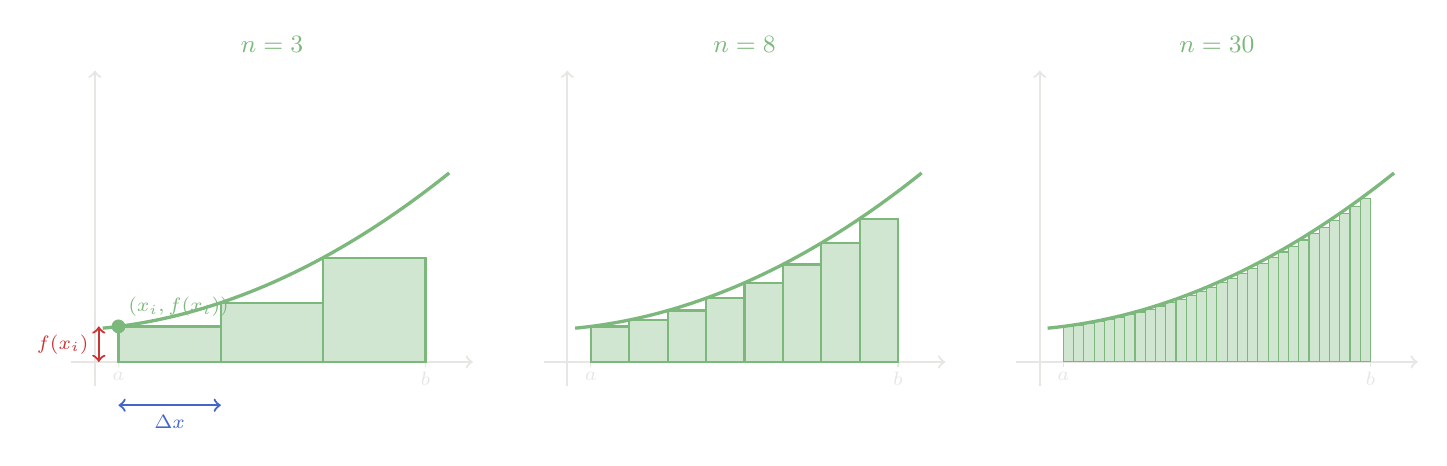
\begin{tikzpicture}

% Curve macro: f(x) = 0.08*(x+0.5)^2 + 0.4  on [0, 4.5] mapped to panel coords
% Panel width = 4cm, height = 3.5cm
% a = 0.3, b = 4.2 in panel coords

\def\fa{0.3}
\def\fb{4.2}
\newcommand{\curvefn}[1]{0.08*(#1+0.5)*(#1+0.5) + 0.4}

% --- Panel 1: n=3 (with annotations) ---
\begin{scope}[shift={(0,0)}]
  \node[anchor=south, accent, font=\bfseries\small] at (2.25,3.8) {$n = 3$};

  % Axes
  \draw[->, lightfg, thick] (-0.3,0) -- (4.8,0);
  \draw[->, lightfg, thick] (0,-0.3) -- (0,3.7);

  % a, b labels
  \node[lightfg, font=\scriptsize, below] at (\fa, 0) {$a$};
  \node[lightfg, font=\scriptsize, below] at (\fb, 0) {$b$};

  % Tick marks
  \draw[lightfg] (\fa, 0.06) -- (\fa, -0.06);
  \draw[lightfg] (\fb, 0.06) -- (\fb, -0.06);

  % Rectangles n=3
  \pgfmathsetmacro{\dx}{(\fb - \fa) / 3}
  \foreach \i in {0,1,2} {
    \pgfmathsetmacro{\xleft}{\fa + \i * \dx}
    \pgfmathsetmacro{\xright}{\xleft + \dx}
    \pgfmathsetmacro{\fval}{\curvefn{\xleft}}
    \fill[accent, opacity=0.35] (\xleft, 0) rectangle (\xright, \fval);
    \draw[accent, thick] (\xleft, 0) rectangle (\xright, \fval);
  }

  % Curve
  \draw[accent, very thick, domain=0.1:4.5, samples=60] plot (\x, {\curvefn{\x}});

  % Annotation: delta-x bracket (first rectangle)
  \pgfmathsetmacro{\xfirst}{\fa}
  \pgfmathsetmacro{\xsecond}{\fa + \dx}
  \draw[bluecol, thick, <->] (\xfirst, -0.55) -- (\xsecond, -0.55)
    node[midway, below, font=\scriptsize, bluecol] {$\Delta x$};

  % Annotation: f(x_i) height arrow (first rectangle)
  \pgfmathsetmacro{\fvali}{\curvefn{\xfirst}}
  \draw[redcol, thick, <->] (\xfirst - 0.25, 0) -- (\xfirst - 0.25, \fvali)
    node[midway, left, font=\scriptsize, redcol] {$f(x_i)$};

  % Annotation: point label
  \fill[accent] (\xfirst, \fvali) circle (2.5pt);
  \node[accent, font=\scriptsize, above right] at (\xfirst, \fvali) {$(x_i, f(x_i))$};
\end{scope}

% --- Panel 2: n=8 ---
\begin{scope}[shift={(6,0)}]
  \node[anchor=south, accent, font=\bfseries\small] at (2.25,3.8) {$n = 8$};

  \draw[->, lightfg, thick] (-0.3,0) -- (4.8,0);
  \draw[->, lightfg, thick] (0,-0.3) -- (0,3.7);
  \node[lightfg, font=\scriptsize, below] at (\fa, 0) {$a$};
  \node[lightfg, font=\scriptsize, below] at (\fb, 0) {$b$};
  \draw[lightfg] (\fa, 0.06) -- (\fa, -0.06);
  \draw[lightfg] (\fb, 0.06) -- (\fb, -0.06);

  \pgfmathsetmacro{\dx}{(\fb - \fa) / 8}
  \foreach \i in {0,...,7} {
    \pgfmathsetmacro{\xleft}{\fa + \i * \dx}
    \pgfmathsetmacro{\xright}{\xleft + \dx}
    \pgfmathsetmacro{\fval}{\curvefn{\xleft}}
    \fill[accent, opacity=0.35] (\xleft, 0) rectangle (\xright, \fval);
    \draw[accent, thick] (\xleft, 0) rectangle (\xright, \fval);
  }

  \draw[accent, very thick, domain=0.1:4.5, samples=60] plot (\x, {\curvefn{\x}});
\end{scope}

% --- Panel 3: n=30 ---
\begin{scope}[shift={(12,0)}]
  \node[anchor=south, accent, font=\bfseries\small] at (2.25,3.8) {$n = 30$};

  \draw[->, lightfg, thick] (-0.3,0) -- (4.8,0);
  \draw[->, lightfg, thick] (0,-0.3) -- (0,3.7);
  \node[lightfg, font=\scriptsize, below] at (\fa, 0) {$a$};
  \node[lightfg, font=\scriptsize, below] at (\fb, 0) {$b$};
  \draw[lightfg] (\fa, 0.06) -- (\fa, -0.06);
  \draw[lightfg] (\fb, 0.06) -- (\fb, -0.06);

  \pgfmathsetmacro{\dx}{(\fb - \fa) / 30}
  \foreach \i in {0,...,29} {
    \pgfmathsetmacro{\xleft}{\fa + \i * \dx}
    \pgfmathsetmacro{\xright}{\xleft + \dx}
    \pgfmathsetmacro{\fval}{\curvefn{\xleft}}
    \fill[accent, opacity=0.35] (\xleft, 0) rectangle (\xright, \fval);
    \draw[accent] (\xleft, 0) rectangle (\xright, \fval);
  }

  \draw[accent, very thick, domain=0.1:4.5, samples=60] plot (\x, {\curvefn{\x}});
\end{scope}

\end{tikzpicture}
\end{document}
